\documentclass[]{elsarticle} %review=doublespace preprint=single 5p=2 column
%%% Begin My package additions %%%%%%%%%%%%%%%%%%%
\usepackage[hyphens]{url}
\usepackage{lineno} % add
\providecommand{\tightlist}{%
  \setlength{\itemsep}{0pt}\setlength{\parskip}{0pt}}

\bibliographystyle{elsarticle-harv}
\biboptions{sort&compress} % For natbib
\usepackage{graphicx}
\usepackage{booktabs} % book-quality tables
%% Redefines the elsarticle footer
%\makeatletter
%\def\ps@pprintTitle{%
% \let\@oddhead\@empty
% \let\@evenhead\@empty
% \def\@oddfoot{\it \hfill\today}%
% \let\@evenfoot\@oddfoot}
%\makeatother

% A modified page layout
\textwidth 6.75in
\oddsidemargin -0.15in
\evensidemargin -0.15in
\textheight 9in
\topmargin -0.5in
%%%%%%%%%%%%%%%% end my additions to header

\usepackage[T1]{fontenc}
\usepackage{lmodern}
\usepackage{amssymb,amsmath}
\usepackage{ifxetex,ifluatex}
\usepackage{fixltx2e} % provides \textsubscript
% use upquote if available, for straight quotes in verbatim environments
\IfFileExists{upquote.sty}{\usepackage{upquote}}{}
\ifnum 0\ifxetex 1\fi\ifluatex 1\fi=0 % if pdftex
  \usepackage[utf8]{inputenc}
\else % if luatex or xelatex
  \usepackage{fontspec}
  \ifxetex
    \usepackage{xltxtra,xunicode}
  \fi
  \defaultfontfeatures{Mapping=tex-text,Scale=MatchLowercase}
  \newcommand{\euro}{€}
\fi
% use microtype if available
\IfFileExists{microtype.sty}{\usepackage{microtype}}{}
\usepackage{color}
\usepackage{fancyvrb}
\newcommand{\VerbBar}{|}
\newcommand{\VERB}{\Verb[commandchars=\\\{\}]}
\DefineVerbatimEnvironment{Highlighting}{Verbatim}{commandchars=\\\{\}}
% Add ',fontsize=\small' for more characters per line
\usepackage{framed}
\definecolor{shadecolor}{RGB}{248,248,248}
\newenvironment{Shaded}{\begin{snugshade}}{\end{snugshade}}
\newcommand{\KeywordTok}[1]{\textcolor[rgb]{0.13,0.29,0.53}{\textbf{#1}}}
\newcommand{\DataTypeTok}[1]{\textcolor[rgb]{0.13,0.29,0.53}{#1}}
\newcommand{\DecValTok}[1]{\textcolor[rgb]{0.00,0.00,0.81}{#1}}
\newcommand{\BaseNTok}[1]{\textcolor[rgb]{0.00,0.00,0.81}{#1}}
\newcommand{\FloatTok}[1]{\textcolor[rgb]{0.00,0.00,0.81}{#1}}
\newcommand{\ConstantTok}[1]{\textcolor[rgb]{0.00,0.00,0.00}{#1}}
\newcommand{\CharTok}[1]{\textcolor[rgb]{0.31,0.60,0.02}{#1}}
\newcommand{\SpecialCharTok}[1]{\textcolor[rgb]{0.00,0.00,0.00}{#1}}
\newcommand{\StringTok}[1]{\textcolor[rgb]{0.31,0.60,0.02}{#1}}
\newcommand{\VerbatimStringTok}[1]{\textcolor[rgb]{0.31,0.60,0.02}{#1}}
\newcommand{\SpecialStringTok}[1]{\textcolor[rgb]{0.31,0.60,0.02}{#1}}
\newcommand{\ImportTok}[1]{#1}
\newcommand{\CommentTok}[1]{\textcolor[rgb]{0.56,0.35,0.01}{\textit{#1}}}
\newcommand{\DocumentationTok}[1]{\textcolor[rgb]{0.56,0.35,0.01}{\textbf{\textit{#1}}}}
\newcommand{\AnnotationTok}[1]{\textcolor[rgb]{0.56,0.35,0.01}{\textbf{\textit{#1}}}}
\newcommand{\CommentVarTok}[1]{\textcolor[rgb]{0.56,0.35,0.01}{\textbf{\textit{#1}}}}
\newcommand{\OtherTok}[1]{\textcolor[rgb]{0.56,0.35,0.01}{#1}}
\newcommand{\FunctionTok}[1]{\textcolor[rgb]{0.00,0.00,0.00}{#1}}
\newcommand{\VariableTok}[1]{\textcolor[rgb]{0.00,0.00,0.00}{#1}}
\newcommand{\ControlFlowTok}[1]{\textcolor[rgb]{0.13,0.29,0.53}{\textbf{#1}}}
\newcommand{\OperatorTok}[1]{\textcolor[rgb]{0.81,0.36,0.00}{\textbf{#1}}}
\newcommand{\BuiltInTok}[1]{#1}
\newcommand{\ExtensionTok}[1]{#1}
\newcommand{\PreprocessorTok}[1]{\textcolor[rgb]{0.56,0.35,0.01}{\textit{#1}}}
\newcommand{\AttributeTok}[1]{\textcolor[rgb]{0.77,0.63,0.00}{#1}}
\newcommand{\RegionMarkerTok}[1]{#1}
\newcommand{\InformationTok}[1]{\textcolor[rgb]{0.56,0.35,0.01}{\textbf{\textit{#1}}}}
\newcommand{\WarningTok}[1]{\textcolor[rgb]{0.56,0.35,0.01}{\textbf{\textit{#1}}}}
\newcommand{\AlertTok}[1]{\textcolor[rgb]{0.94,0.16,0.16}{#1}}
\newcommand{\ErrorTok}[1]{\textcolor[rgb]{0.64,0.00,0.00}{\textbf{#1}}}
\newcommand{\NormalTok}[1]{#1}
\usepackage{graphicx}
% We will generate all images so they have a width \maxwidth. This means
% that they will get their normal width if they fit onto the page, but
% are scaled down if they would overflow the margins.
\makeatletter
\def\maxwidth{\ifdim\Gin@nat@width>\linewidth\linewidth
\else\Gin@nat@width\fi}
\makeatother
\let\Oldincludegraphics\includegraphics
\renewcommand{\includegraphics}[1]{\Oldincludegraphics[width=\maxwidth]{#1}}
\ifxetex
  \usepackage[setpagesize=false, % page size defined by xetex
              unicode=false, % unicode breaks when used with xetex
              xetex]{hyperref}
\else
  \usepackage[unicode=true]{hyperref}
\fi
\hypersetup{breaklinks=true,
            bookmarks=true,
            pdfauthor={},
            pdftitle={Food-web complexity alters the fitness landscape of an insect herbivore},
            colorlinks=true,
            urlcolor=blue,
            linkcolor=magenta,
            pdfborder={0 0 0}}
\urlstyle{same}  % don't use monospace font for urls
\setlength{\parindent}{0pt}
\setlength{\parskip}{6pt plus 2pt minus 1pt}
\setlength{\emergencystretch}{3em}  % prevent overfull lines
\setcounter{secnumdepth}{0}
% Pandoc toggle for numbering sections (defaults to be off)
\setcounter{secnumdepth}{0}
% Pandoc header


\usepackage[nomarkers]{endfloat}

\begin{document}
\begin{frontmatter}

  \title{Food-web complexity alters the fitness landscape of an insect herbivore}
    \author[a,b]{Matthew A. Barbour\corref{c1}}
   \ead{matthew.barbour@ieu.uzh.ch} 
   \cortext[c1]{Corresponding Author}
    \author[a,c]{Christopher J. Greyson-Gaito}
  
  
    \author[a]{Arezoo Sootodeh}
  
  
    \author[d]{Brendan Locke}
  
  
    \author[b]{Jordi Bascompte}
  
  
      \address[a]{University of British Columbia, Department of Zoology, 6270 University
Blvd., Vancouver, BC, V6T 1Z4, Canada}
    \address[b]{University of Zurich, Department of Evolutionary Biology and
Environmental Studies, Winterthurerstrasse 190, Zurich, 8057,
Switzerland}
    \address[c]{University of Guelph, Department of Integrative Biology, 50 Stone Rd.
East, Guelph, ONT, N1G 2W1, Canada}
    \address[d]{Humboldt State University, Department of Biological Sciences, 1 Harpst
St., Arcata, CA, 95521, USA}
  
  \begin{abstract}
  Studies of natural selection and fitness landscapes usually treat the
  network of interacting species as a ``black box''. Given that the loss
  of biodiversity is simplifying the structure of ecological networks,
  there is a pressing need to answer the question: how does network
  complexity affect natural selection and the fitness landscape of
  associated species? To answer this question, we conducted a field
  experiment that manipulated the complexity of a food web associated with
  a galling insect herbivore. To maintain complex food webs, we allowed
  the entire community of natural enemies to attack insect galls on 64
  plants in a common garden setting. To create simple food webs, we
  excluded a guild of three larval parasitoids by bagging galls on 64
  different plants; therefore, mortality in this treatment was primarily
  due to a single egg parasitoid that attacks prior to gall formation. We
  then measured herbivore survival as a function of three key gall traits
  in each treatment. We found that more traits were under selection in the
  simple vs.~complex food web. This occurred because different parasitoid
  species impose different selection pressures on gall traits, thereby
  minimizing relative fitness differences among insect galls with
  different phenotypes. Our work suggests that more complex food webs
  allow phenotypic variation to persist, which could facilitate subsequent
  adaptive evolution to environmental change.
  \end{abstract}
  
 \end{frontmatter}

\section{Introduction}\label{introduction}

Biological diversity -- from genes, to phenotypes, to species -- has and
continues to be shaped by the interplay between ecological and
evolutionary processes. Much of this biological diversity has been
molded by natural selection arising from species interactions, such as
resource competition (Schluter (2000)), mutualisms (Jordano (1987)), and
predation (Abrams (2000)). While there is clear evidence that pairwise
interactions can drive evolution, we also know that most species
interact with multiple species in an ecological community. Understanding
how evolutionary dynamics unfold in a community context is challenging
and eminently theoretical (Mcpeek (2017), Mazancourt, Johnson, and
Barraclough (2008), Guimarães et al. (2017), Nuismer, Jordano, and
Bascompte (2013)). Given the rapid loss of species diversity we are
experiencing throughout the world (cite), we are in urgent need of work
that makes and tests predictions for how the loss of species will affect
the evolutionary process in natural communities.

Predicting the evolutionary consequences of species loss first requires
an understanding of the concommitant change in the species-interaction
networks. Knowing the interaction network is crucial because the loss of
biodiversity, in and of itself, will not alter evolution -- it is the
associated loss of ecological interactions that will affect evolutionary
change (Janzen (1974)). For a network of directly connected species, we
would expect that the loss of species to result in a loss of network
complexity. Network complexity is a property that describes the
diversity of interactions in an ecological community (Banasek-Richter et
al. (2009)). Thus, all else equal, species loss will decrease the
diversity of interactions, resulting in a more simple network.

Predicting how a change in network complexity will alter evolution also
requires an understanding of the relationship between network structure
and the adaptive landscape. The adaptive landscape (i.e.~fitness
landscape or selective surface) describes the relationship between the
average trait value of a population and its average fitness (cite
Arnold). For a trophic network, such as a food web, changes in network
complexity can shape the adaptive landscape of constituent species in at
least two ways. First, if a more diverse community of consumers is more
efficient at suppressing resource densities (Ives, Cardinale, and Snyder
(2005)), then this will result in lower mean fitness of the resource
population. A reduction in mean fitness, all else equal, will intensify
natural selection (Hunter et al. (2018)) and thus could speed up the
rate of evolutionary change. On the other hand, if consumers are
functionally distinct, then more diverse communities can dampen the
strength of selection. This is because each consumer has a different
functional relationship with resource traits. In addition, there is a
reduced probability in interacting with a specific consumer species in a
more diverse community. Thus, a more diverse consumer community may
impose more diffuse selection across the adaptive landscape.

Here, we provide a quantitative test of how the loss of species
diversity -- and concomittant loss of network complexity -- shapes the
adaptive landscape of a consitutent species in a natural community. We
conducted a field experiment that manipulated the diversity of insect
parasitoids that were able to impose selection on the insect herbivore,
\emph{Iteomyia salicisverruca}. The larva of this herbivore species
induces tooth-shaped galls when they feed on the developing leaves of
willow trees (\emph{Salix} sp., Russo (2006)). Prior work with this
study system has shown that there is directional selection for larger
galls, likely because larger galls provide a refuge from parasitoid
attack (Barbour et al. (2016)). However, there is also evidence that
each parasitoid species imposes differential selection on gall traits
(Barbour et al. (2016)). Taken together, our aim is to provide evidence
for how the simplification of natural communities affects the adaptive
potential of constituent species.

\section{Materials \& Methods}\label{materials-methods}

\subsection{Study Site}\label{study-site}

We conducted our study within a four-year old common garden of coastal
willow (\emph{Salix hookeriana}) located at Humboldt Bay National
Wildlife Refuge (HBNWR) (40°40'53``N, 124°12'4''W) near Loleta,
California, USA. This common garden consists of 26 different willow
genotypes that were collected from a single population of willows
growing around Humboldt Bay. Stem cuttings of each genotype (25
replicates per genotypes) were planted in a completely randomized design
in two hectares of a former cattle pasture at HBNWR. Willows in our
garden begin flowering in February and reach their peak growth in early
August. During this study, willows had reached 5 - 9m in height. Further
details on the genotyping and planting of the common garden are
available in Barbour et al. (2015).

\subsection{Food-Web Manipulation}\label{food-web-manipulation}

We setup our food-web manipulation across 128 plants soon after galls
began developing on \emph{S. hookeriana} in early June of 2013. These
128 plants came from eight different plant genotypes, spanning the range
of trait variation observed in this willow population (Barbour et al.
(2015)). On treatment plants (8 replicates per genotype), we enclosed 14
galled leaves with 10x15cm organza bags (ULINE, Pleasant Prairie, WI,
USA) to exclude three parasitoid species that attack during larva
development (hereafter larval parasitoids). This treatment did not
exclude the egg parasitoid \emph{Platygaster} sp. which attacks prior to
gall initiation (note that in Cecidomyiid midges, larva initiate gall
development CITE). On control plants (8 replicates per genotype), we
used flagging tape to mark 14 galled leaves per plant, allowing the full
suite of parasitoids to attack \emph{Iteomyia}. Marking galls with
flagging tape ensured that we compared control and treatment galls with
similar phenology when we collected galls later in the season. Our
food-web manipulation altered the average number of trophic interactions
that \emph{Iteomyia} was exposed to from BLANK on control plants to
BLANK on treatment plants. Thus, we refer to galls on control plants as
being exposed to a `complex' food web, whereas galls on treatment plants
were exposed to a `simple' food web. In late August, we collected marked
and bagged galls from each plant, placed them into 30 mL vials and kept
them in the lab for 4 months at room temperature. We then opened galls
under a dissecting scope and determined whether larva survived to
pupation (our measure of fitness) or were parasitized.

\subsection{Measuring Gall Traits}\label{measuring-gall-traits}

We collected data on three different traits that we anticipated would
experience selection based on our previous work (Barbour et al. (2016))
and others work with Cecidomyiid midges (Weis, Price, and Lynch (1983),
Heath, Abbot, and Stireman (2018)). First, we measured gall diameter as
the size of each gall chamber to the nearest 0.01 mm at its maximum
diameter (perpendicular to the direction of plant tissue growth). Our
previous work has shown that a larger gall diameter provides a refuge
for larva from parasitoid attack (Barbour et al. (2016)). Second, we
measured the clutch size of adult female midges by counting the number
of chambers in each gall (Weis, Price, and Lynch (1983)). All larva
collected from the same multi-chambered gall were scored with the same
clutch size. Third, we measured female preference for oviposition
(egg-laying) sites as the density of larva observed on a plant. The
measurement of larval densities on plants in the field is a commonly
used index for measuring oviposition preference (Gripenberg et al.
(2010)), although caution must be taken in inferring `preference'
(Singer (1986)). This is because larval densities can be influenced by
processes other than preference. For example, if an ovipositing female
is not exposed to the full spectrum of plant types (in this case
genotypes), then it is difficult to infer whether patterns of larval
densities are actually due to preference. Also, observed larval
densities could be influenced by egg predation.\\
While we recognize these limitations, a couple of aspects of our study
system likely alleviate these limitations. For example, since our data
comes from a randomized placement of willow genotypes in a common
garden, there is no consistent bias in which willow genotypes that
females are exposed to while searching for oviposition sites. Although
we cannot control for egg predation, this source of mortality appears to
play comparatively minor role in determining the mortality of galling
insects (Hawkins, Cornell, and Hochberg (1997)). To quantify female
preference (gall density), we randomly sampled five branches per tree
and summed the number of individual gall chambers observed. We converted
these counts to a measure of gall density per 100 shoots by counting the
number of shoots on the last branch we sampled. All larva collected from
the same plant were scored with the same female preference.

\subsection{Statistical Analyses}\label{statistical-analyses}

To characterize the shape of the fitness landscape in simple and complex
food webs, we fit separate statistical models to quantify individual
selection surfaces acting on each trait. We used generalized linear
mixed models (GLMMs, Bolker et al. (2009)) with larval survival (0 or 1)
as our response variable and measure of fitness. In our full model, we
specified linear and quadratic terms for each gall trait as well as
linear interaction terms between each gall trait as fixed effects in the
statistical models. To account for the correlated structure of clutch
size (gall level) and female preference (plant level) as well as any
other independent effects of willow genotype on larval survival, we
specified gall ID nested within plant ID nested within plant genotype as
random intercepts in our statistical models. Since we were interested in
characterizing the fitness landscape -- the relationship between mean
trait values and population mean fitness -- we assumed the mean value of
our random effects (i.e.~setting them to zero) to estimate selection
gradients. We then used the method of Frederic J Janzen and Hal S Stearn
(1998) to calculate directional (\(\beta_{z_i}\)), quadratic
(\(\gamma_{z_i}\)), and correlational (\(\gamma_{z_i,z_j}\)) selection
gradients and used parametric bootstrapping (1000 replicates) to
calculate their 95\% confidence intervals (Bolker et al. (2009)). We
estimated directional selection gradients by excluding quadratic terms
and statistical interactions in the model. To test whether selection
gradients differed between treatments, we used our bootstrapped
estimates to calculate the probability that selection gradients in the
simple food web were larger/smaller than in the complex food web
(i.e.~the p-value). Together, we had survival estimates for 1,306 larva,
607 galls, 111 plants, and 8 plant genotypes. We report estimated
selection gradients and the 95\% confidence intervals in parentheses.
All analyses and visualizations were conducted in R (R Core Team
(2018)).

\begin{Shaded}
\begin{Highlighting}[]
\NormalTok{## Summarize Control Selection Gradients ----}
\NormalTok{summary_beta_control <-}\StringTok{ }\KeywordTok{data.frame}\NormalTok{(}
  \DataTypeTok{Phenotype =} \KeywordTok{c}\NormalTok{(}\StringTok{"Gall diameter"}\NormalTok{, }\StringTok{"Clutch size"}\NormalTok{, }\StringTok{"Female preference"}\NormalTok{),}
  \DataTypeTok{Food_Web =} \StringTok{"Complex"}\NormalTok{,}
  \DataTypeTok{Model =} \StringTok{"GLMM"}\NormalTok{,}
  \DataTypeTok{Type =} \StringTok{"Beta"}\NormalTok{,}
  \DataTypeTok{Estimate =} \KeywordTok{round}\NormalTok{(}\KeywordTok{Beta_avg_grad}\NormalTok{(beta_control),}\DecValTok{3}\NormalTok{),}
  \DataTypeTok{lower_2.5 =} \KeywordTok{round}\NormalTok{(}\KeywordTok{apply}\NormalTok{(boot_beta_control}\OperatorTok{$}\NormalTok{t, }\DecValTok{2}\NormalTok{, }\DataTypeTok{FUN =} \ControlFlowTok{function}\NormalTok{(bootstraps) }\KeywordTok{quantile}\NormalTok{(bootstraps, }\FloatTok{0.025}\NormalTok{)),}\DecValTok{3}\NormalTok{),}
  \DataTypeTok{upper_97.5 =} \KeywordTok{round}\NormalTok{(}\KeywordTok{apply}\NormalTok{(boot_beta_control}\OperatorTok{$}\NormalTok{t, }\DecValTok{2}\NormalTok{, }\DataTypeTok{FUN =} \ControlFlowTok{function}\NormalTok{(bootstraps) }\KeywordTok{quantile}\NormalTok{(bootstraps, }\FloatTok{0.975}\NormalTok{)),}\DecValTok{3}\NormalTok{)) }

\CommentTok{# doubled quadratic estimates to make comparable to directional selection gradients (Stinchcombe et al. 2008, Evolution)}
\NormalTok{summary_quad_control <-}\StringTok{ }\KeywordTok{data.frame}\NormalTok{(}
  \DataTypeTok{Phenotype =} \KeywordTok{c}\NormalTok{(}\StringTok{"Gall diameter"}\NormalTok{, }\StringTok{"Clutch size"}\NormalTok{, }\StringTok{"Female preference"}\NormalTok{),}
  \DataTypeTok{Food_Web =} \StringTok{"Complex"}\NormalTok{,}
  \DataTypeTok{Model =} \StringTok{"GLMM"}\NormalTok{,}
  \DataTypeTok{Type =} \StringTok{"Quadratic"}\NormalTok{,}
  \DataTypeTok{Estimate =} \DecValTok{2}\OperatorTok{*}\KeywordTok{round}\NormalTok{(}\KeywordTok{Beta_avg_grad}\NormalTok{(quad_control),}\DecValTok{3}\NormalTok{)[}\OperatorTok{-}\KeywordTok{c}\NormalTok{(}\DecValTok{1}\OperatorTok{:}\DecValTok{3}\NormalTok{)],}
  \DataTypeTok{lower_2.5 =} \DecValTok{2}\OperatorTok{*}\KeywordTok{round}\NormalTok{(}\KeywordTok{apply}\NormalTok{(boot_quad_control}\OperatorTok{$}\NormalTok{t, }\DecValTok{2}\NormalTok{, }\DataTypeTok{FUN =} \ControlFlowTok{function}\NormalTok{(bootstraps) }\KeywordTok{quantile}\NormalTok{(bootstraps, }\FloatTok{0.025}\NormalTok{)),}\DecValTok{3}\NormalTok{)[}\OperatorTok{-}\KeywordTok{c}\NormalTok{(}\DecValTok{1}\OperatorTok{:}\DecValTok{3}\NormalTok{)],}
  \DataTypeTok{upper_97.5 =} \DecValTok{2}\OperatorTok{*}\KeywordTok{round}\NormalTok{(}\KeywordTok{apply}\NormalTok{(boot_quad_control}\OperatorTok{$}\NormalTok{t, }\DecValTok{2}\NormalTok{, }\DataTypeTok{FUN =} \ControlFlowTok{function}\NormalTok{(bootstraps) }\KeywordTok{quantile}\NormalTok{(bootstraps, }\FloatTok{0.975}\NormalTok{)),}\DecValTok{3}\NormalTok{)[}\OperatorTok{-}\KeywordTok{c}\NormalTok{(}\DecValTok{1}\OperatorTok{:}\DecValTok{3}\NormalTok{)]) }

\NormalTok{summary_corr_control <-}\StringTok{ }\KeywordTok{data.frame}\NormalTok{(}
  \DataTypeTok{Phenotype =} \KeywordTok{c}\NormalTok{(}\StringTok{"Diam,Clutch"}\NormalTok{, }\StringTok{"Diam,Pref"}\NormalTok{, }\StringTok{"Clutch,Pref"}\NormalTok{),}
  \DataTypeTok{Food_Web =} \StringTok{"Complex"}\NormalTok{,}
  \DataTypeTok{Model =} \StringTok{"GLMM"}\NormalTok{,}
  \DataTypeTok{Type =} \StringTok{"Correlational"}\NormalTok{,}
  \DataTypeTok{Estimate =} \KeywordTok{round}\NormalTok{(}\KeywordTok{Beta_avg_grad}\NormalTok{(corr_control),}\DecValTok{3}\NormalTok{)[}\OperatorTok{-}\KeywordTok{c}\NormalTok{(}\DecValTok{1}\OperatorTok{:}\DecValTok{6}\NormalTok{)],}
  \DataTypeTok{lower_2.5 =} \KeywordTok{round}\NormalTok{(}\KeywordTok{apply}\NormalTok{(boot_corr_control}\OperatorTok{$}\NormalTok{t, }\DecValTok{2}\NormalTok{, }\DataTypeTok{FUN =} \ControlFlowTok{function}\NormalTok{(bootstraps) }\KeywordTok{quantile}\NormalTok{(bootstraps, }\FloatTok{0.025}\NormalTok{)),}\DecValTok{3}\NormalTok{)[}\OperatorTok{-}\KeywordTok{c}\NormalTok{(}\DecValTok{1}\OperatorTok{:}\DecValTok{6}\NormalTok{)],}
  \DataTypeTok{upper_97.5 =} \KeywordTok{round}\NormalTok{(}\KeywordTok{apply}\NormalTok{(boot_corr_control}\OperatorTok{$}\NormalTok{t, }\DecValTok{2}\NormalTok{, }\DataTypeTok{FUN =} \ControlFlowTok{function}\NormalTok{(bootstraps) }\KeywordTok{quantile}\NormalTok{(bootstraps, }\FloatTok{0.975}\NormalTok{)),}\DecValTok{3}\NormalTok{)[}\OperatorTok{-}\KeywordTok{c}\NormalTok{(}\DecValTok{1}\OperatorTok{:}\DecValTok{6}\NormalTok{)]) }


\NormalTok{## Summarize Treatment Selection Gradients ----}
\NormalTok{summary_beta_treatment <-}\StringTok{ }\KeywordTok{data.frame}\NormalTok{(}
  \DataTypeTok{Phenotype =} \KeywordTok{c}\NormalTok{(}\StringTok{"Gall diameter"}\NormalTok{, }\StringTok{"Clutch size"}\NormalTok{, }\StringTok{"Female preference"}\NormalTok{),}
  \DataTypeTok{Food_Web =} \StringTok{"Simple"}\NormalTok{,}
  \DataTypeTok{Model =} \StringTok{"GLMM"}\NormalTok{,}
  \DataTypeTok{Type =} \StringTok{"Beta"}\NormalTok{,}
  \DataTypeTok{Estimate =} \KeywordTok{round}\NormalTok{(}\KeywordTok{Beta_avg_grad}\NormalTok{(beta_treatment),}\DecValTok{3}\NormalTok{),}
  \DataTypeTok{lower_2.5 =} \KeywordTok{round}\NormalTok{(}\KeywordTok{apply}\NormalTok{(boot_beta_treatment}\OperatorTok{$}\NormalTok{t, }\DecValTok{2}\NormalTok{, }\DataTypeTok{FUN =} \ControlFlowTok{function}\NormalTok{(bootstraps) }\KeywordTok{quantile}\NormalTok{(bootstraps, }\FloatTok{0.025}\NormalTok{)),}\DecValTok{3}\NormalTok{),}
  \DataTypeTok{upper_97.5 =} \KeywordTok{round}\NormalTok{(}\KeywordTok{apply}\NormalTok{(boot_beta_treatment}\OperatorTok{$}\NormalTok{t, }\DecValTok{2}\NormalTok{, }\DataTypeTok{FUN =} \ControlFlowTok{function}\NormalTok{(bootstraps) }\KeywordTok{quantile}\NormalTok{(bootstraps, }\FloatTok{0.975}\NormalTok{)),}\DecValTok{3}\NormalTok{)) }

\CommentTok{# doubled quadratic estimates to make comparable to directional selection gradients (Stinchcombe et al. 2008, Evolution)}
\NormalTok{summary_quad_treatment <-}\StringTok{ }\KeywordTok{data.frame}\NormalTok{(}
  \DataTypeTok{Phenotype =} \KeywordTok{c}\NormalTok{(}\StringTok{"Gall diameter"}\NormalTok{, }\StringTok{"Clutch size"}\NormalTok{, }\StringTok{"Female preference"}\NormalTok{),}
  \DataTypeTok{Food_Web =} \StringTok{"Simple"}\NormalTok{,}
  \DataTypeTok{Model =} \StringTok{"GLMM"}\NormalTok{,}
  \DataTypeTok{Type =} \StringTok{"Quadratic"}\NormalTok{,}
  \DataTypeTok{Estimate =} \DecValTok{2}\OperatorTok{*}\KeywordTok{round}\NormalTok{(}\KeywordTok{Beta_avg_grad}\NormalTok{(quad_treatment),}\DecValTok{3}\NormalTok{)[}\OperatorTok{-}\KeywordTok{c}\NormalTok{(}\DecValTok{1}\OperatorTok{:}\DecValTok{3}\NormalTok{)],}
  \DataTypeTok{lower_2.5 =} \DecValTok{2}\OperatorTok{*}\KeywordTok{round}\NormalTok{(}\KeywordTok{apply}\NormalTok{(boot_quad_treatment}\OperatorTok{$}\NormalTok{t, }\DecValTok{2}\NormalTok{, }\DataTypeTok{FUN =} \ControlFlowTok{function}\NormalTok{(bootstraps) }\KeywordTok{quantile}\NormalTok{(bootstraps, }\FloatTok{0.025}\NormalTok{)),}\DecValTok{3}\NormalTok{)[}\OperatorTok{-}\KeywordTok{c}\NormalTok{(}\DecValTok{1}\OperatorTok{:}\DecValTok{3}\NormalTok{)],}
  \DataTypeTok{upper_97.5 =} \DecValTok{2}\OperatorTok{*}\KeywordTok{round}\NormalTok{(}\KeywordTok{apply}\NormalTok{(boot_quad_treatment}\OperatorTok{$}\NormalTok{t, }\DecValTok{2}\NormalTok{, }\DataTypeTok{FUN =} \ControlFlowTok{function}\NormalTok{(bootstraps) }\KeywordTok{quantile}\NormalTok{(bootstraps, }\FloatTok{0.975}\NormalTok{)),}\DecValTok{3}\NormalTok{)[}\OperatorTok{-}\KeywordTok{c}\NormalTok{(}\DecValTok{1}\OperatorTok{:}\DecValTok{3}\NormalTok{)]) }

\NormalTok{summary_corr_treatment <-}\StringTok{ }\KeywordTok{data.frame}\NormalTok{(}
  \DataTypeTok{Phenotype =} \KeywordTok{c}\NormalTok{(}\StringTok{"Diam,Clutch"}\NormalTok{, }\StringTok{"Diam,Pref"}\NormalTok{, }\StringTok{"Clutch,Pref"}\NormalTok{),}
  \DataTypeTok{Food_Web =} \StringTok{"Simple"}\NormalTok{,}
  \DataTypeTok{Model =} \StringTok{"GLMM"}\NormalTok{,}
  \DataTypeTok{Type =} \StringTok{"Correlational"}\NormalTok{,}
  \DataTypeTok{Estimate =} \KeywordTok{round}\NormalTok{(}\KeywordTok{Beta_avg_grad}\NormalTok{(corr_treatment),}\DecValTok{3}\NormalTok{)[}\OperatorTok{-}\KeywordTok{c}\NormalTok{(}\DecValTok{1}\OperatorTok{:}\DecValTok{6}\NormalTok{)],}
  \DataTypeTok{lower_2.5 =} \KeywordTok{round}\NormalTok{(}\KeywordTok{apply}\NormalTok{(boot_corr_treatment}\OperatorTok{$}\NormalTok{t, }\DecValTok{2}\NormalTok{, }\DataTypeTok{FUN =} \ControlFlowTok{function}\NormalTok{(bootstraps) }\KeywordTok{quantile}\NormalTok{(bootstraps, }\FloatTok{0.025}\NormalTok{)),}\DecValTok{3}\NormalTok{)[}\OperatorTok{-}\KeywordTok{c}\NormalTok{(}\DecValTok{1}\OperatorTok{:}\DecValTok{6}\NormalTok{)],}
  \DataTypeTok{upper_97.5 =} \KeywordTok{round}\NormalTok{(}\KeywordTok{apply}\NormalTok{(boot_corr_treatment}\OperatorTok{$}\NormalTok{t, }\DecValTok{2}\NormalTok{, }\DataTypeTok{FUN =} \ControlFlowTok{function}\NormalTok{(bootstraps) }\KeywordTok{quantile}\NormalTok{(bootstraps, }\FloatTok{0.975}\NormalTok{)),}\DecValTok{3}\NormalTok{)[}\OperatorTok{-}\KeywordTok{c}\NormalTok{(}\DecValTok{1}\OperatorTok{:}\DecValTok{6}\NormalTok{)]) }

\KeywordTok{bind_rows}\NormalTok{(summary_beta_control, summary_beta_treatment) }\OperatorTok\StringTok{ }\KeywordTok{arrange}\NormalTok{(Phenotype)}
\end{Highlighting}
\end{Shaded}

\begin{verbatim}
## Warning in bind_rows_(x, .id): Unequal factor levels: coercing to character
\end{verbatim}

\begin{verbatim}
## Warning in bind_rows_(x, .id): binding character and factor vector,
## coercing into character vector

## Warning in bind_rows_(x, .id): binding character and factor vector,
## coercing into character vector
\end{verbatim}

\begin{verbatim}
##           Phenotype Food_Web Model Type Estimate lower_2.5 upper_97.5
## 1       Clutch size  Complex  GLMM Beta    0.043    -0.044      0.106
## 2       Clutch size   Simple  GLMM Beta   -0.091    -0.243     -0.012
## 3 Female preference  Complex  GLMM Beta   -0.093    -0.246      0.051
## 4 Female preference   Simple  GLMM Beta   -0.232    -0.906     -0.362
## 5     Gall diameter  Complex  GLMM Beta    0.442     0.418      0.604
## 6     Gall diameter   Simple  GLMM Beta    0.328     0.191      0.319
\end{verbatim}

\begin{Shaded}
\begin{Highlighting}[]
\KeywordTok{bind_rows}\NormalTok{(summary_quad_control, summary_quad_treatment) }\OperatorTok\StringTok{ }\KeywordTok{arrange}\NormalTok{(Phenotype)}
\end{Highlighting}
\end{Shaded}

\begin{verbatim}
## Warning in bind_rows_(x, .id): Unequal factor levels: coercing to character

## Warning in bind_rows_(x, .id): binding character and factor vector,
## coercing into character vector

## Warning in bind_rows_(x, .id): binding character and factor vector,
## coercing into character vector
\end{verbatim}

\begin{verbatim}
##           Phenotype Food_Web Model      Type Estimate lower_2.5 upper_97.5
## 1       Clutch size  Complex  GLMM Quadratic   -0.056    -0.228      0.118
## 2       Clutch size   Simple  GLMM Quadratic   -0.110    -0.440      0.094
## 3 Female preference  Complex  GLMM Quadratic    0.180     0.028      0.276
## 4 Female preference   Simple  GLMM Quadratic   -0.076    -0.548      0.266
## 5     Gall diameter  Complex  GLMM Quadratic    0.066    -0.070      0.188
## 6     Gall diameter   Simple  GLMM Quadratic    0.064    -0.122      0.232
\end{verbatim}

\begin{Shaded}
\begin{Highlighting}[]
\KeywordTok{bind_rows}\NormalTok{(summary_corr_control, summary_corr_treatment) }\OperatorTok\StringTok{ }\KeywordTok{arrange}\NormalTok{(Phenotype)}
\end{Highlighting}
\end{Shaded}

\begin{verbatim}
## Warning in bind_rows_(x, .id): Unequal factor levels: coercing to character

## Warning in bind_rows_(x, .id): binding character and factor vector,
## coercing into character vector

## Warning in bind_rows_(x, .id): binding character and factor vector,
## coercing into character vector
\end{verbatim}

\begin{verbatim}
##     Phenotype Food_Web Model          Type Estimate lower_2.5 upper_97.5
## 1 Clutch,Pref  Complex  GLMM Correlational    0.041    -0.054      0.142
## 2 Clutch,Pref   Simple  GLMM Correlational    0.006    -0.110      0.119
## 3 Diam,Clutch  Complex  GLMM Correlational   -0.044    -0.144      0.060
## 4 Diam,Clutch   Simple  GLMM Correlational   -0.093    -0.278      0.009
## 5   Diam,Pref  Complex  GLMM Correlational   -0.105    -0.245      0.008
## 6   Diam,Pref   Simple  GLMM Correlational   -0.012    -0.114      0.114
\end{verbatim}

\begin{figure}
\centering
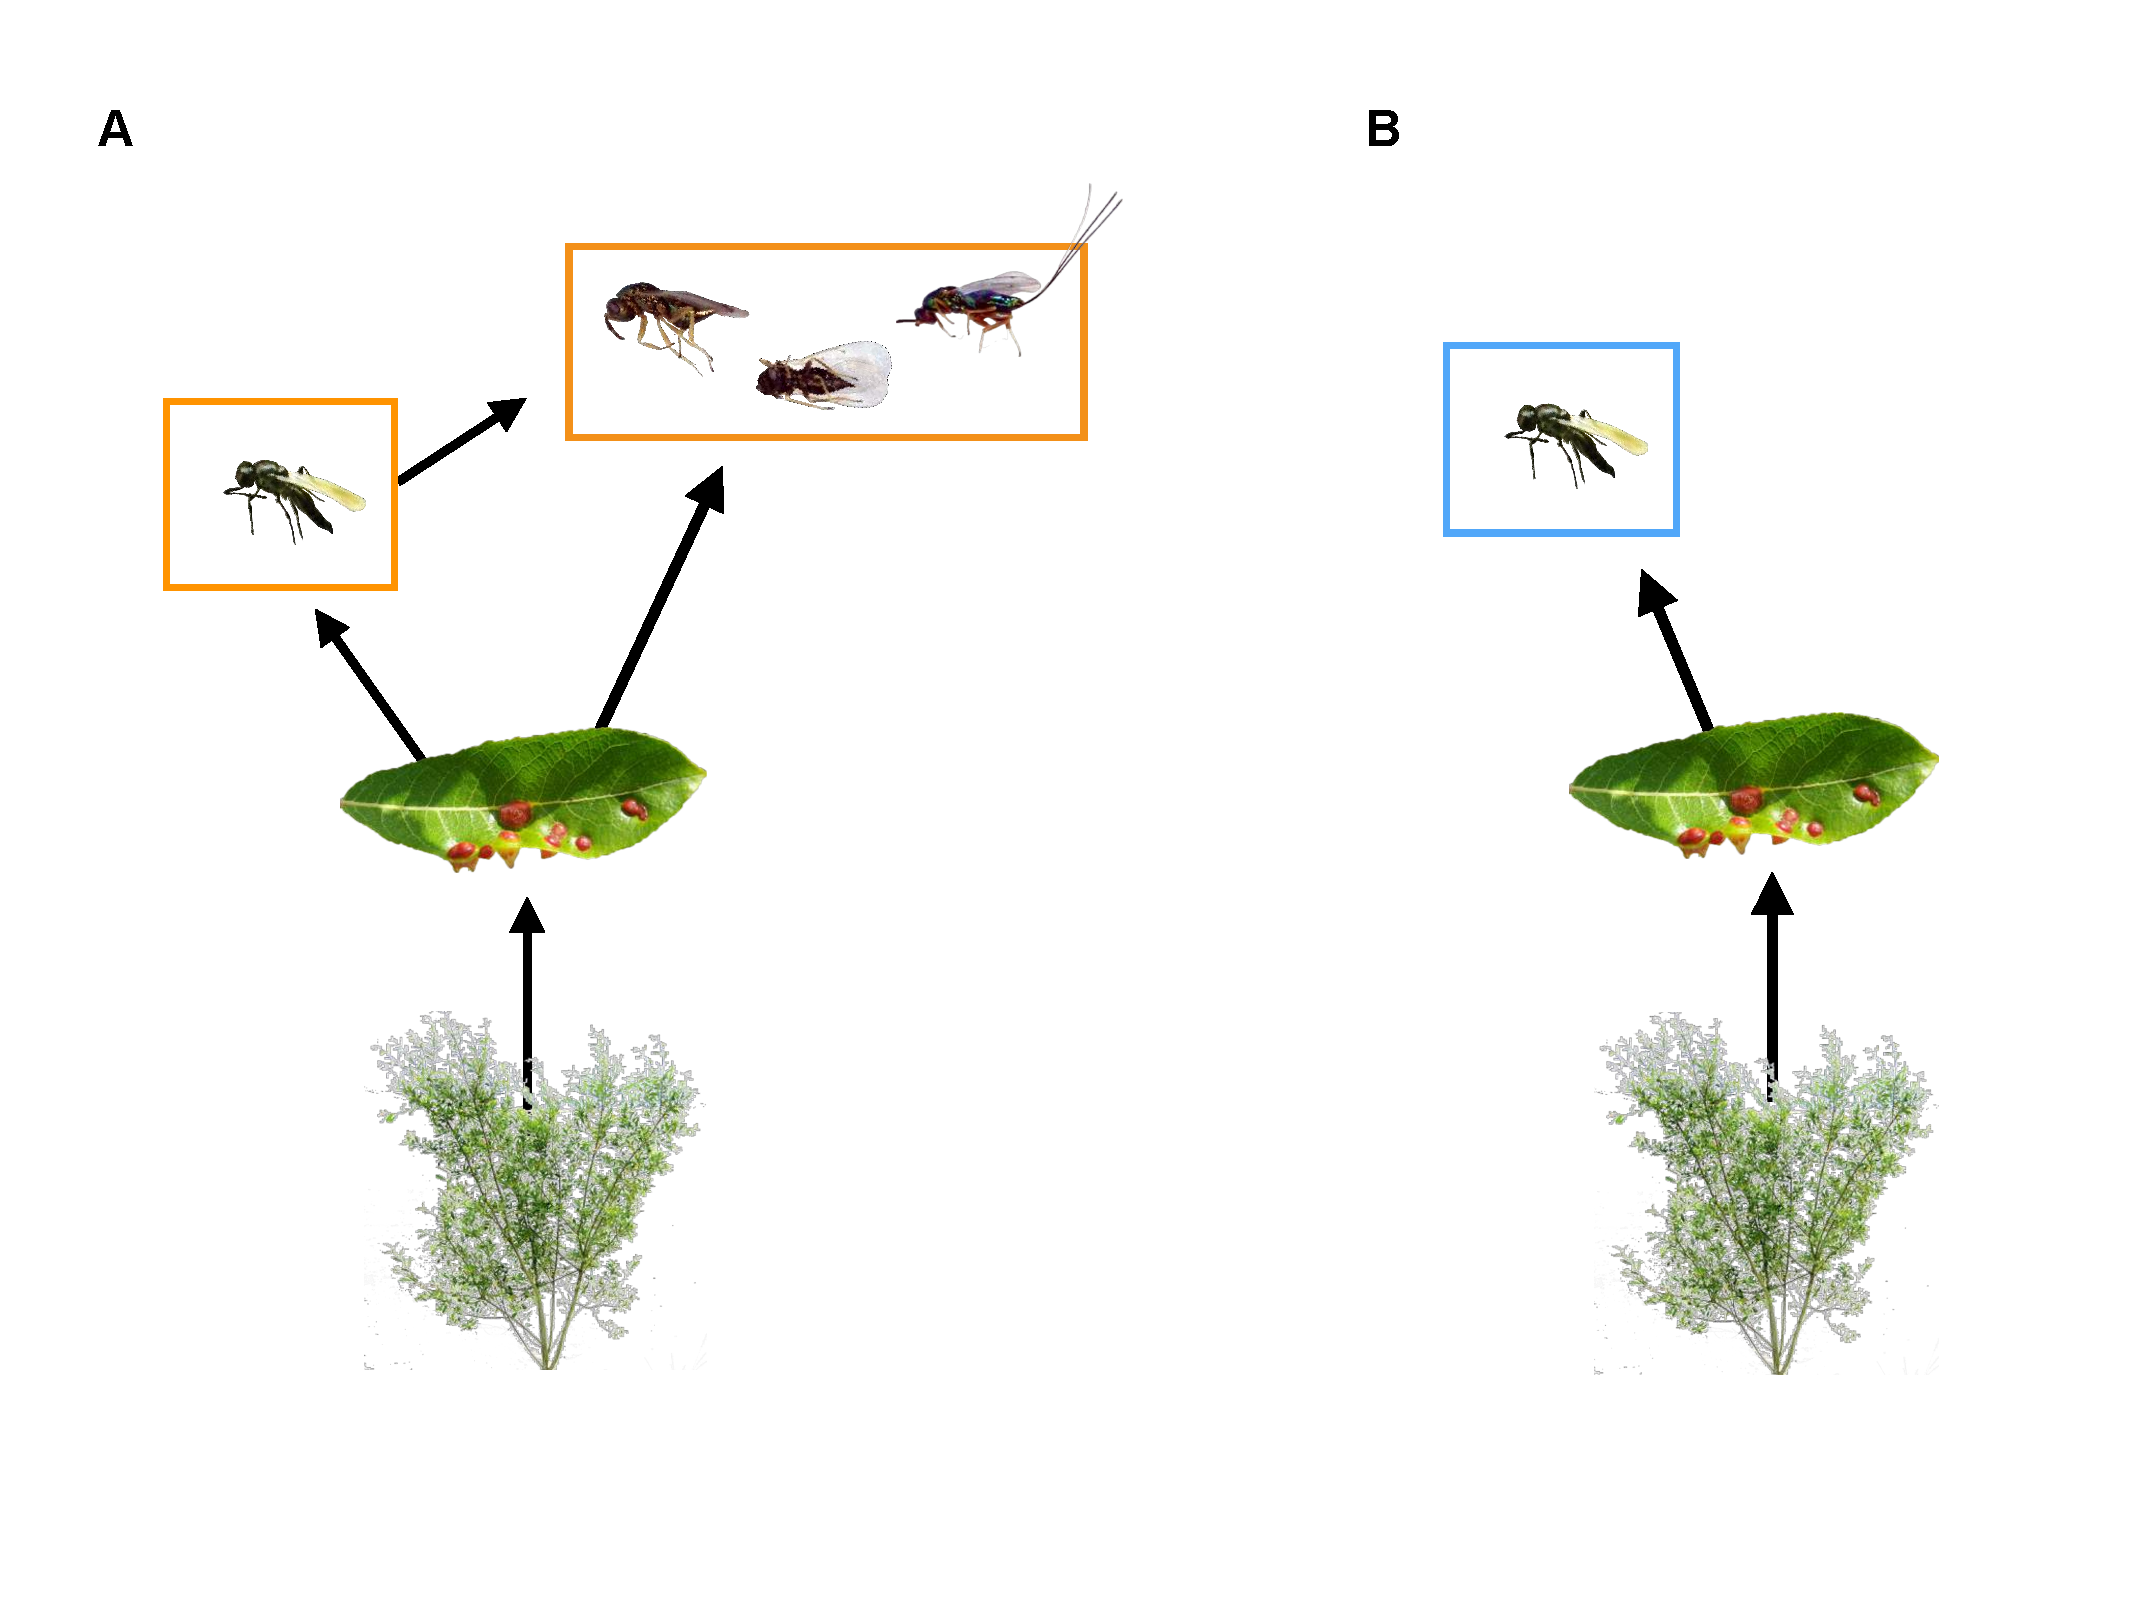
\includegraphics{complex_simple_foodwebs_compressed.pdf}
\caption{Illustrations of complex (A) and simple (B) food webs
associated with the insect herbivore, \emph{Iteomyia salicisverruca}.
Black arrows denote `who-eats-whom' in this network of trophic
interactions.}
\end{figure}

\section{Results}\label{results}

Two key patterns emerged from our analyses. First, fewer phenotypic
traits were under selection in the complex vs.~simple food web. In both
complex and simple food webs, gall diameter was under strong directional
selection, with larger galls resulting in higher larval survival
(complex \(\beta_{diam}=\) 0.442 {[}0.418,0.604{]} ; simple
\(\beta_{diam}=\) 0.328 {[}0.191,0.319{]} )(Fig.
\ref{fig:Univariate_Landscapes}A). In simple food webs, both clutch size
and female preference experience directional selection, with smaller
clutch sizes (\(\beta_{clutch}=\) -0.091 {[}-0.243,-0.012{]} and weaker
preferences (\(\beta_{pref}=\) -0.232 {[}-0.906,-0.362{]} ) resulting in
higher larval survival (blue lines in Fig.
\ref{fig:Univariate_Landscapes}B,C). In contrast, there was no evidence
of selection on clutch size (\(\beta_{clutch}=\) 0.043
{[}-0.044,0.106{]} ) or female preference (\(\beta_{pref}=\) -0.093
{[}-0.246,0.051{]} ) in complex food webs (orange lines in Fig.
\ref{fig:Univariate_Landscapes}B,C). The absence of selection on clutch
size and female preference was likely a result of conflicting selection
pressures imposed by each guild of parasitoids due to their different
functional relationships with gall traits. Together, these different
patterns of selection resulted in an ideal combination of traits having
higher fitness in the simple food web (large diameter, smaller clutches,
weaker preference), whereas there was a larger combination of trait
values that had equal fitness in the complex food web (Fig.
\ref{fig:Multivariate_Landscapes}). We did not find any strong evidence
for nonlinear or correlational selection gradients acting on gall traits
in either food-web treatment. The second major pattern was that the
overall intensity of selection was stronger in the complex vs.~simple
food web. This result appeared to be driven by selection on gall
diameter in the complex food web, which was more than 1.3 \(\times\)
larger than any other selection gradient in our analyses.

\begin{figure}
\centering
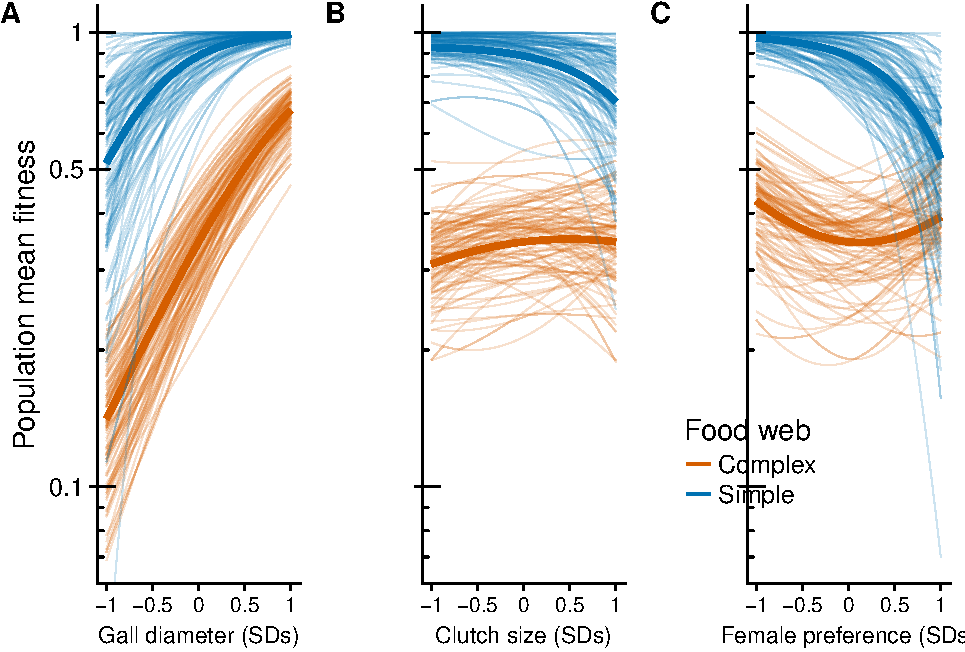
\includegraphics{elsevier_test_files/figure-latex/Univariate_Landscapes-1.pdf}
\caption{\label{fig:Univariate_Landscapes}Selection gradients acting on
gall traits in complex vs.~simple food webs. Each panel corresponds to a
different gall trait: gall diameter (A); clutch size (B); and female
preference (C). Solid lines represent the estimated gradients in complex
(orange) and simple (blue) food webs. Transparent lines represent
bootstrapped replicates (n=100) to show the uncertainty in estimated
gradients. Note that only 100 bootstraps are displayed here, but that
inferences are based on 1,000 bootstrapped samples.}
\end{figure}

\begin{figure}
\centering
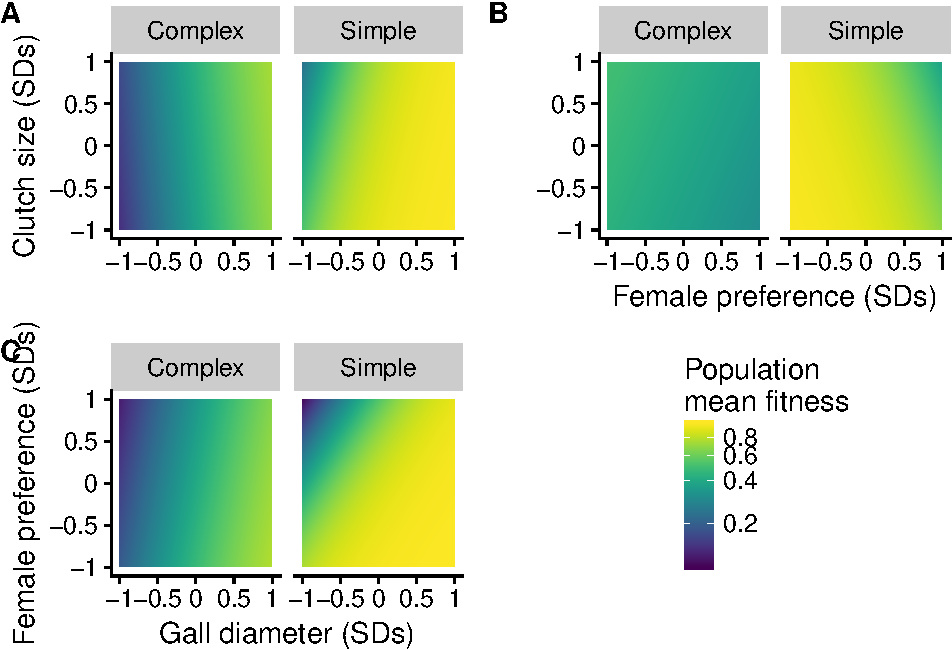
\includegraphics{elsevier_test_files/figure-latex/Multivariate_Landscapes-1.pdf}
\caption{\label{fig:Multivariate_Landscapes}Fitness landscapes of gall
traits in complex vs.~simple food webs. Each panel corresponds to a
different combination of traits: clutch size and gall diameter (A);
clutch size and female preference (B); female preference and gall
diameter (C). Note that traits for all plots range 1 SD below and above
the mean (=0).}
\end{figure}

\section{Discussion}\label{discussion}

Our key finding was that the adaptive landscape was less constrained in
the complex vs.~simple food web. These fewer constraints arise from
conflicting selection pressures imposed by different parasitoid guilds,
resulting in fewer traits under selection in the complex food web. At
the same time, we observed an overall greater intensity of selection in
the complex food web, suggesting that trait evolution can be faster in
complex vs.~simple food webs. Our observation that natural selection was
more constrained and less intense in simple vs.~complex food webs
suggests that the loss of biodiversity could constrain the adaptive
potential of interacting species by reducing genetic and phenotypic
variation in multiple traits.

Current theory suggests that when the number of selective constrains is
less than the number of genetic constraints (i.e.~some genetically
variable traits are selective neutral), there are multiple positions on
the landscape that confer equal fitness (Lande 1981; Lande and Arnold
1985). In this scenario, trait differences between populations may
simply be due to neutral processes (e.g.~genetic drift and mutation)
moving trait values of the population. For our system, we currently lack
quantitative estimates of genetic variation in our traits, although work
with other species of galling insects has shown that gall diameter
(Abramhson, Heath's work), clutch size (look to Weiss' work), and
oviposition preference (Abrahmson's work?) are genetically variable. We
encourage others to examine how changes in community context will alter
selection on multiple traits.

One interesting result of our work was that the overall intensity of
selection appeared to be larger in complex food webs. This result was
driven by the large selection gradient acting on gall diameter in
complex vs.~simple food webs. This difference in selection intensity is
likely not driven by a difference in the ecological relationship between
gall diameter and parasitoid attack (i.e.~slope), but actually a result
of the lower mean fitness of \emph{Iteomyia} in the complex food web.
This lower mean fitness is not surprising ---we excluded an entire guild
of parasitoids from attacking the insect. But this more intense
selection pressure may simply represent a transient dynamic. This is
because we would expect the egg-parasitoid \emph{Platygaster} to
increase in abundance over time once its intraguild predator has been
removed. While our results suggest that this wouldn't affect the slope
of the relationship, the higher abundance of the egg parasitoid would
likely reduce the mean fitness of \emph{Iteomyia}, thus increasing the
selection gradient acting on gall diameter closer to what we observed in
the complex food web. We don't expect it to fully compensate, given that
the larval parasitoids exhibit a different functional relationship with
gall traits, and thus we expect a more diverse community of primary
parasitoids to generally impose greater parasitism pressure, a factor
that appears to be a general trend in parasitoid community (Hawkins
citation) and likely for other consumers (Ives and Cardinale Ecology
Letters).

Our study focused on quantifying the direct effects of changes in
network complexity on the fitness landscape; however, changes in network
complexity may have pervasive indirect effects via coevolution or by
initiating evolutionary cascades. In our system, we observed that
excluding the guild of larval parasitoids altered selection on both the
basal resource (\emph{Iteomyia}) and the intraguild prey
(\emph{Platygaster}). GIVE DETAILS AND SUGGEST A POTENTIAL EVOLUTIONARY
CASCADE.

Our study manipulated food-web complexity and examined changes in the
fitness landscape of species embedded within this network. However,
other studies have also examined, at least theoretically, how changes in
the diversity of competitive communities affects evolution. These
studies have generally suggested that the diversity of competitors may
actually constrain the adaptive landscape, a finding that stands in
contrast to our results. NEED TO REVIEW THESE PAPERS TO SEE HOW ITS
DIFFERENT.

We suggest that by explicitly focusing on network structure, we can
predict how changes in biodiversity will affect the adaptive potential
of constituent species. A network allows a powerful representation of
the `community context', lending predictive power to how changes in
network structure (either due to loss of species or links), will alter
natural selection and consequently evolutionary change. Our results also
suggest that losing biodiversity may not just have consequences at the
community level, but also population-level consequences that may
actually constrain adaptation to changing environments. This argues that
changes in network complexity may not only affect the robustness of
communities, but also that of constituent populations to future
environmental change.

\section*{References}\label{references}
\addcontentsline{toc}{section}{References}

\hypertarget{refs}{}
\hypertarget{ref-Abrams2000}{}
Abrams, Peter A. 2000. ``The Evolution of Predator-Prey Interactions:
Theory and Evidence.'' \emph{Annu. Rev. Ecol. Syst.} 31. Annual Reviews:
79--105.

\hypertarget{ref-Banasek-Richter2009}{}
Banasek-Richter, Carolin, Louis-Félix Bersier, Marie-France Cattin,
Richard Baltensperger, Jean-Pierre Gabriel, Yves Merz, Robert E
Ulanowicz, et al. 2009. ``Complexity in Quantitative Food Webs.''
\emph{Ecology} 90 (6): 1470--7.

\hypertarget{ref-Barbour2016}{}
Barbour, Matthew A, Miguel A Fortuna, Jordi Bascompte, Joshua R
Nicholson, Riitta Julkunen-Tiitto, Erik S Jules, and Gregory M
Crutsinger. 2016. ``Genetic Specificity of a Plant--insect Food Web:
Implications for Linking Genetic Variation to Network Complexity.''
\emph{Proceedings of the National Academy of Sciences} 113 (8). National
Acad Sciences: 2128--33.

\hypertarget{ref-Barbour2015}{}
Barbour, Matthew A, Mariano A Rodriguez-Cabal, Elizabeth T Wu, Riitta
Julkunen-Tiitto, Carol E Ritland, Allyson E Miscampbell, Erik S Jules,
and Gregory M Crutsinger. 2015. ``Multiple Plant Traits Shape the
Genetic Basis of Herbivore Community Assembly.'' \emph{Funct. Ecol.} 29
(8): 995--1006.

\hypertarget{ref-Bolker2009}{}
Bolker, Benjamin M, Mollie E Brooks, Connie J Clark, Shane W Geange,
John R Poulsen, M Henry H Stevens, and Jada-Simone S White. 2009.
``Generalized Linear Mixed Models: A Practical Guide for Ecology and
Evolution.'' \emph{Trends Ecol. Evol.} 24 (3): 127--35.

\hypertarget{ref-Janzen1998}{}
Frederic J Janzen and Hal S Stearn. 1998. ``Logistic Regression for
Empirical Studies of Multivariate Selection.'' \emph{Evolution} 52 (6):
1564--71.

\hypertarget{ref-Gripenberg2010}{}
Gripenberg, Sofia, Peter J Mayhew, Mark Parnell, and Tomas Roslin. 2010.
``A Meta-Analysis of Preference-Performance Relationships in
Phytophagous Insects.'' \emph{Ecol. Lett.} 13 (3): 383--93.

\hypertarget{ref-Guimaraes2017}{}
Guimarães, Paulo R, Jr, Mathias M Pires, Pedro Jordano, Jordi Bascompte,
and John N Thompson. 2017. ``Indirect Effects Drive Coevolution in
Mutualistic Networks.'' \emph{Nature} 550 (7677): 511--14.

\hypertarget{ref-Hawkins1997}{}
Hawkins, Bradford A, Howard V Cornell, and Michael E Hochberg. 1997.
``Predators, Parasitoids, and Pathogens as Mortality Agents in
Phytophagous Insect Populations.'' \emph{Ecology} 78 (7). Ecological
Society of America: 2145--52.

\hypertarget{ref-Heath2018}{}
Heath, Jeremy J, Patrick Abbot, and John O Stireman 3rd. 2018.
``Adaptive Divergence in a Defense Symbiosis Driven from the Top down.''
\emph{Am. Nat.} 192 (1): E21--E36.

\hypertarget{ref-Hunter2018}{}
Hunter, Darren C, Josephine M Pemberton, Jill G Pilkington, and Michael
B Morrissey. 2018. ``Quantification and Decomposition of
Environment-Selection Relationships.'' \emph{Evolution}, March.

\hypertarget{ref-Ives2005}{}
Ives, Anthony R, Bradley J Cardinale, and William E Snyder. 2005. ``A
Synthesis of Subdisciplines: Predator--prey Interactions, and
Biodiversity and Ecosystem Functioning.'' \emph{Ecol. Lett.} 8 (1).
Blackwell Science Ltd: 102--16.

\hypertarget{ref-Janzen1974}{}
Janzen, Daniel. 1974. ``The Deflowering of Central America.''
\emph{Natural History} 83 (January): 49--53.

\hypertarget{ref-Jordano1987}{}
Jordano, Pedro. 1987. ``Patterns of Mutualistic Interactions in
Pollination and Seed Dispersal: Connectance, Dependence Asymmetries, and
Coevolution.'' \emph{Am. Nat.} 129 (5): 657--77.

\hypertarget{ref-De_Mazancourt2008}{}
Mazancourt, C de, E Johnson, and T G Barraclough. 2008. ``Biodiversity
Inhibits Species' Evolutionary Responses to Changing Environments.''
\emph{Ecol. Lett.} 11 (4): 380--88.

\hypertarget{ref-McPeek2017}{}
Mcpeek, Mark A. 2017. \emph{Evolutionary Community Ecology}. Princeton
University Press.

\hypertarget{ref-Nuismer2013}{}
Nuismer, Scott L, Pedro Jordano, and Jordi Bascompte. 2013.
``Coevolution and the Architecture of Mutualistic Networks.''
\emph{Evolution} 67 (2): 338--54.

\hypertarget{ref-R2018}{}
R Core Team. 2018. \emph{R: A Language and Environment for Statistical
Computing}. Vienna, Austria: R Foundation for Statistical Computing.
\url{https://www.R-project.org/}.

\hypertarget{ref-Russo2006}{}
Russo, Ron. 2006. \emph{Field Guide to Plant Galls of California and
Other Western States}. 1st ed. University of California Press.

\hypertarget{ref-Schluter2000}{}
Schluter, Dolph. 2000. ``Ecological Character Displacement in Adaptive
Radiation.'' \emph{Am. Nat.} 156 (S4): S4--S16.

\hypertarget{ref-Singer1986}{}
Singer, Michael C. 1986. ``The Definition and Measurement of Oviposition
Preference in Plant-Feeding Insects.'' In \emph{Insect-Plant
Interactions}, edited by James R Miller and Thomas A Miller, 65--94. New
York, NY: Springer New York.

\hypertarget{ref-Weis1983}{}
Weis, Arthur E, Peter W Price, and Michael Lynch. 1983. ``Selective
Pressures on Clutch Size in the Gall Maker Asteromyia Carbonifera.''
\emph{Ecology} 64 (4). Ecological Society of America: 688--95.

\end{document}


